\chapter{Lane Detection, Tracking and SDLP Calculation}  \label{kap:sdlp}

Everybody in this world is concerned about safety. The people those who go out from
one place to other, expect to reach safely. Without any sudden incidents which may come 
through externally by road accidents while travelling. We can avoid the road accidents by 
using improved driving assistances. Therefore, a system that provides a means of warning 
the driver to the danger has the potential to save a considerable number of lives. One of the 
main technologies involved in these tasks is computer vision, which become a powerful tool for 
sensing the environment and detect road boundaries. Lane detection and object detection plays 
vital role for accidents. For human vision and human intelligence the task of lane detection and 
object detection changes due to variations in the road conditions. Sometimes it is very easy to 
detect with the human eyes but in some conditions due to externals effects the human intelligent 
have detection problems. 

Driver inattention has been a major focus of driver safety research (Klauer et al., 2006; 
Ranney et al., 2000; Wang et al.,1996). In recent years however, naturalistic studies have made 
it possible to gain additional insights on driver behavior and have actually demonstrated that 
78\% of crashes and 65\% of near crashes are driver inattention related (Klauer et al., 2006). The 
main causes of collisions can be driver error, drowsiness, impaired driving due to alcohol/drugs 
or distractions due to a phone call or tuning the radio. Many studies have shown that driver 
inattention can influence lane-keeping ability. One of the main source of making this analysis on 
vehicle control is the standard deviation of lateral position (SDLP), ie, the
amount of ``weaving''
of the car.

The basic purpose of developing this android app as a proof of concept is to help
researchers in domain of ergonomics to investigate driver's behavior in different scenarios. We 
are proposing a system which acquires the front view using an android phone camera mounted 
on the vehicle then applying few processes in order to detect the lanes. We are using an open 
source code for lane detection \cite{lane-code} to provide the baseline functionality which is developed to run 
on PC. Code is ported to Android NDK project and then improved further and features added as 
per our requirement.

\section{Lane Detection and Tracking}

Lane departure warning system is a mechanism designed to warn a driver when the 
vehicle begins to move out of his lane (unless a turn signal is on in that
direction) on freeways and arterial roads. Lane detection algorithms detect lane markings and the edges
of the road, and estimate the vehicle position in the lane. A lane detection system must be
able to pick out all manner of markings from cluttered roadways and filter them to produce a
reliable estimate of the vehicle position and trajectory relative to the lane.

A typical lane tracking process includes:

\begin{itemize}
    \item Video acquisition.
    \item Matrix downsampling and set Region of Interest (ROI).
    \item Line Detection.
    \item Lane Detection.
    \item Lane Tracking.
\end{itemize}

\begin{figure}
\begin{center}
    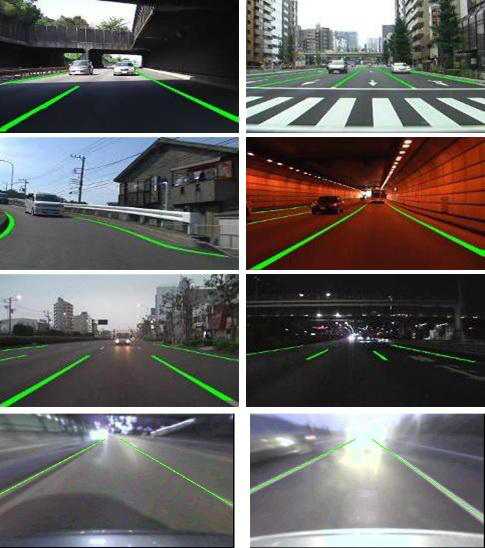
\includegraphics[scale=0.6]{img/lane1.png}
\end{center}
\caption{Examples of lane detection and tracking}
\label{fig:lane1}
\end{figure}

We are using some assumptions for our solution as it is a prototype and also we
something which is manageable but still suffice the need of a good proof of concept. 

\begin{itemize}
\item Road is assumed to be of fixed lane width and constant texture so that
searching for parallel lane markings is efficient.
\item It is a constraint to process the varying painted and the unpainted roads or
the dash and the solid paint line roads. Its good to assume a continuous or dashed but bright
lane markings.
\item It is a constraint to handle the curved roads and good assumption is that the
roads are straight without intersections and bumps.
\item Experimental results are not constraint to be robust against noise, shadows
due to trees/ building, and illumination variations in the captured road images. Other issues
are due to wet road, direct sunshine on the cameras, tunnels and bridges' shadows.
Avoidance of these possibilities simplifies road geometry reconstruction. 
\item Other vehicles on the path partly occlude the visibility of the road and
    therefore also of road markings. The road is assumed to be one way but can by 2 lane road.
\item A constant weather and lighting conditions are assumed. More precise, the 
    video stream that will be used for training and testing are going to be taken 
    during daylight and without rain or fog.
\end{itemize}

\subsection{Video acquisition}

There are many sources for the video acquisition in field of signal processing.
The main important one is vision based approach. In our project, we are using
Android phone camera instead of an external camera and video stream recorded by camera would
be used as input. Now we have really powerful android phones with normally 5 MP camera
which is good enough for Computer Vision applications. In our case, phone is mounted on the
dashboard in a landscape position where it can get a good view of the road surface and the
vanishing point of road should be somewhere at center.

\subsection{Matrix downsampling, Grey scaling and setting Region of Interest (ROI)}

Computation of Image processing algorithms is very resource oriented task on
Smartphones but there are several proven techniques which can be used to limit
the enormous space of frames in which each window has to pass the classifier. Otherwise we
were facing extremely poor frames per second (fps) rate. 

One of the techniques is to downsample the matrix by reducing the size of image
frame.  It reduces quality which is a tradeoff but it doesn't affect significantly on
ultimate output. We are reducing the size of each input frame by 1/4 and then upsampling it again by
factor of 4 before displaying it back on screen. This concept is also referred as Scale Space.

\begin{figure}
\begin{center}
    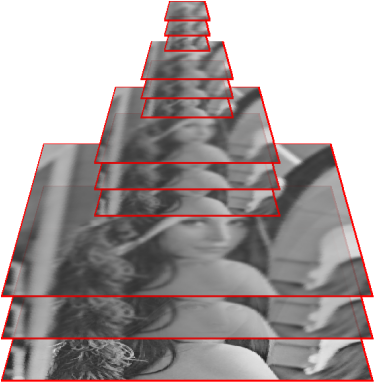
\includegraphics[scale=0.6]{img/lane2.png}
\end{center}
\caption{Scale Space Demonstration}
\label{fig:lane2}
\end{figure}

The captured image is also converted to gray scale to make method faster, less
computations, and less sensitive to scene condition \cite{lane2}. The other influential
technique is setting a custom Region of Interest (ROI) to limit the search for
lane markers to a specific region of the image to speed things up. This helps in
segmentation of the space and remove all areas that we are certain of not
containing the lane markings. It creates a binary mask and only detect in
windows that lie in the smallest bounding box of our blobs of possible
candidates.

\begin{figure}
\begin{center}
    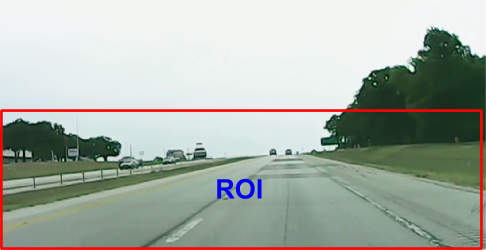
\includegraphics[scale=0.6]{img/lane3.png}
\end{center}
\caption{Region of Interest selection}
\label{fig:lane3}
\end{figure}

\subsection{Canny Edge Detection}

Canny edge detection is one of the edge detection methods that is used to find all the edge points in the image and output is a binary map. Canny runs a gradient on the image to find sharp changes in the pixel intensities. These are likely contours in the image. The output is then just a binary map that shows you where the contours of the image are located. 

In this step, we use Canny edge detection to find lane boundaries in the frame. Canny edge detection basically uses gradient vector of an intensity image. Lane boundaries have high contrast in the image, and this feature yields high values of gradient vector by which we can find the edge direction, which is orthogonal to gradient vector. It is one of the best and efficient methods among many edge detection methods \cite{lane3}.

\begin{figure}
\begin{center}
    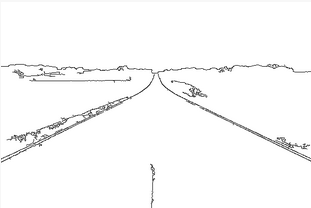
\includegraphics[scale=0.6]{img/lane4.png}
\end{center}
\caption{Example of a contour image}
\label{fig:lane4}
\end{figure}

\subsection{Hough Transform}

The Hough transform is a technique which can be used to isolate features of a particular shape within an image. Developed by Paul Hough in 1962 and patented by IBM, the transform requires the desired features to be specified in some parametric form, the classical Hough transform is most commonly used for the detection of regular curves such as lines, circles, ellipses, etc. The main advantage of the Hough transform technique is that it is tolerant of gaps in feature boundary descriptions and is relatively unaffected by image noise.

Let's take an image (figure~\ref{fig:lane5}) with two lines A and B. Obviously both lines are each made of its own set of pixels laying on a straight line. Now, one way or another we need to learn our software which pixels are on a straight line and, if so, to what line they belong to.

\begin{figure}
\begin{center}
    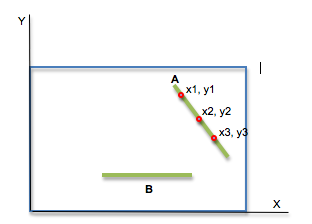
\includegraphics[scale=0.6]{img/lane5.png}
\end{center}
\caption{Line creation from points.}
\label{fig:lane5}
\end{figure}

\begin{figure}
\begin{center}
    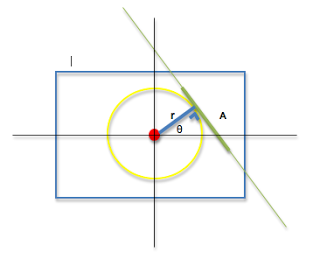
\includegraphics[scale=0.6]{img/lane6.png}
\end{center}
\caption{The transformation.}
\label{fig:lane6}
\end{figure}

The trick of the Hough Transformation is to represent lines in a polar coordinate system (see figure~\ref{fig:lane6}), or in this case, also called "Hough Space". 

The important thing in figure~\ref{fig:lane6} is that we imagine a line from the center (the blue line) which is perpendicular to the line we want to find (the green line) and we call the distance from the center $r$ and $\theta$(theta) is the angle to the $X$ axis (the angle between the blue line and the $X$ axis).

The transformation from any $(x, y)$ pixel in figure~\ref{fig:lane1} to the $(r, \theta)$ representation in figure~\ref{fig:lane6} is the following:

\begin{equation}
    r = x \cos(\theta) + y \sin(\theta) 
\end{equation}

Now, if you lean back and think a bit about Fig 6. Every possible line can be represented by a unique $r$ and $\theta$. And further, every pixel on a given line will transform to the exact same $r$ and $\theta$ for that line. And this is immediately the most important aspect of the whole Hough stuff. 

\subsection{Lane Detection}

Lane detection phase uses the Hough Lines function to extract line segments in the image based on Hough transform. The parameters are thresholded version of contours, the Hough Lines which become the output and the Hough Vote. The Hough Vote is an important parameter because it influence the accuracy and time taken by the algorithm. It is basically the minimum number of points passing through a line. So the higher value of Hough Vote means the smaller inaccurate lines would be rejected and helps in removing the noise but the trade-off is performance. We have added a slider input ( 0 - 200 ) before the start of the application instead of making it fixed so that user can change Hough Vote value which can help in investigation of the researcher.

The Hough Lines object finds Cartesian coordinates of lines that are described by rho and theta pairs. The lines are filtered on basis of theta and lines with theta values between 4 degrees and 84 degrees or between 95 degrees and 180 degrees are allowed only to pass through. This is to ensure that we have the lines which are more probably the true lanes. Then we want to find the point of intersection i.e\ $x$ and $y$ so that we can plot the line by connecting these points.

\begin{equation}
    x = \frac{r - y\sin(\theta)}{\cos(\theta)} \hspace{1cm} y = \frac{r - x
    \cos(\theta)}{\sin(\theta)}
\end{equation}

\begin{figure}
\begin{center}
    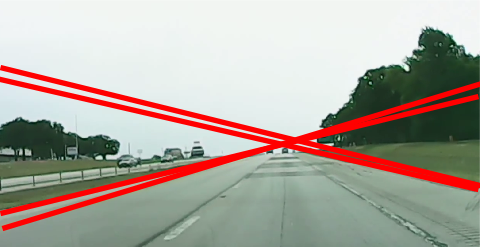
\includegraphics[scale=0.6]{img/lane7.png}
\end{center}
\caption{After applying Hough Transform and Hough Lines}
\label{fig:lane7}
\end{figure}

The problem with this current progress is that we can not find the endpoints of the lane that is also known as vanishing point of lane. For this, Probabilistic Hough Transform \cite{lane4} is used which is pretty much the same as regular Hough Transform but finds the end of each line as shown in the diagram below.


\begin{figure}
\begin{center}
    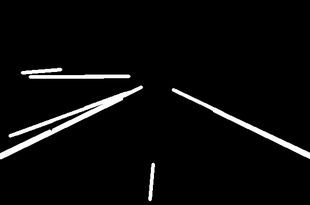
\includegraphics[scale=0.6]{img/lane8.png}
\end{center}
\caption{shows the output of Probabilistic Hough Transform with end points of lane}
\label{fig:lane8}
\end{figure}

The regular transform does not find endpoints and the probabilistic tends to find several other lines that is not required. To solve this problem, a bitwise addition of two images is done. The final output looks like the image below.

\begin{figure}
\begin{center}
    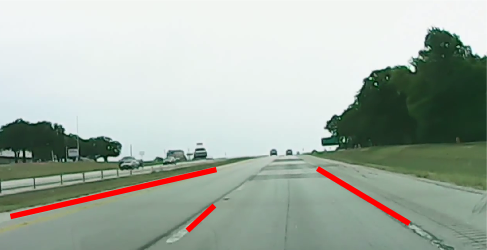
\includegraphics[scale=0.6]{img/lane9.png}
\end{center}
\caption{Shows final output after bitwise addition}
\label{fig:lane9}
\end{figure}

\section{SDLP calculation and Ergonomics}

Our project aims is to develop an android app which will help researchers in investigating and evaluating different driving behaviors in different situations from ergonomics perspective. Many studies have shown that driver inattention can influence lane-keeping ability and hence road accidents. Ergonomics researchers intent to investigate how the car interior can be a reason to distract driver and cause inattention with eyes-off-road. Research has shown that after accounting for driving speed and lane width, the eyes-off-road significantly increased the standard deviation of lane position (SDLP). Visual related distractions occur when drivers need to divert their eyes away from the roadway such as when texting, tuning radio, selecting the playlist etc. 

SDLP stands for standard deviation of lateral position and is considered the primary outcome measure of vehicle control. The secondary outcome measure is the standard deviation of speed (SDS). Since SDLP increment may ultimately result in lane crossings into the road shoulder and adjacent traffic lane, it can also be regarded as a potential index of driving safety. It is considered an international standard of evaluation in the on-the-road driving test around the globe. 


\begin{figure}
\begin{center}
    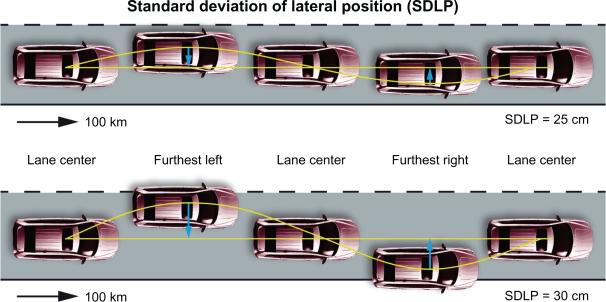
\includegraphics[scale=0.6]{img/lane10.png}
\end{center}
\caption{SDLP demonstrated}
\label{fig:lane10}
\end{figure}

\subsection{Lateral position estimation}

Lateral position refers to the relationship of the correct position of car in lane to a real position of car in the lane. The difference between the true position of car and the actual position of car in lane gives an understanding of how much is driver deviating. This can be directly computed from the distance between the vehicle and the lane marker under the assumption of a fixed lane width (3.56 m) and a known vehicle width (1.52 m). 

In our case, car's position is equivalent to the value of $x$ coordinate of the line detected in the final output. We have defined a scale of values ranging from 450 to 100 for our test video which involves single lane. The selection of this video has many reasons for training and testing. It involves lane switching of driver, there are very few cars on road, the lane boundaries are pretty clear without any shadows and the video is made in daytime so there's enough light. During the training phase, the scale was defined for both lanes. The hypothesis used is that the lanes which are visible in the smartphone camera view actually define the position of car in the lane. Thats why SDLP in our case is just an estimate. 

\subsection{Calculating SDLP}

formula, table of values, results, graphs

The SDLP is calculated the following way:

\begin{itemize}
    \item Calculate the mean lateral position (MLP) for the entire drive 
    \item Calculate the standard deviation of the MLP (= SDLP) across all of the samples taken
\end{itemize}

The equation to calculate a standard deviation is:
When $X$ is the lateral position (determined for each valid data point) with a
mean value $\mu$:

\begin{equation}
    MLP[X] = \mu
    \label{eq:lane1}
\end{equation}

In equation~\ref{eq:lane1}, MLP (mean lateral position) denotes the average of
$X$. The standard deviation of $X$ is the quantity:

\begin{equation}
    SLDP = \sqrt{MLP[(X - \mu)^2]}
\end{equation}

In other words, SDLP is the square root of the variance of $X$, i.e., it is the
square root of the average value of $(X - \mu)^2$.

The following graph shows average values of SDLP calculated from a demo video. The mean value is around 0.80 which is a poor estimation and the reason is that boundary detection is sometimes very inaccurate. The noise data has a negative impact on the dataset. 


\begin{figure}
\begin{center}
    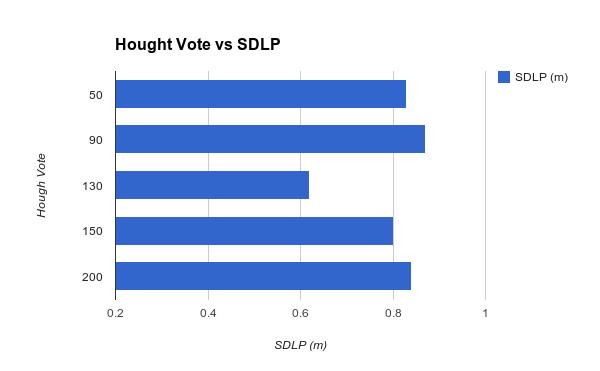
\includegraphics[scale=0.6]{img/lane11.png}
\end{center}
\label{fig:lane11}
\end{figure}

\section{Implementation and Evaluation}

For implementing this proof of concept, we are using Android SDK and Android NDK platform. For computer vision operations, OpenCV Library is used and languages include Java and C++. 

Project Structure :-

\begin{figure}
    \centering\small
    \begin{minipage}[t]{\linewidth}
        \dirtree{%
            .1 Application/.
            .2 jni : Conventional location for C/C++ source code.
            .3 Android.mk : sub-makefile that describes the C++ static libraries and *.so files.
            .3 Application.mk : contains settings that apply to all the C/C++ code.
            .3 LaneDetector.cpp : main cpp file that handles everything.
            .3 linefinder.h : class file that implements lane detection functions.
            .3 LaneCalculations.cpp : implements sdlp functions.
            .3 LaneCalculations.h : class file for sdlp functions.
            .2 res : Conventional location for Android XML resource files.
            .3 src : Conventional location for Android Java source code.
            .3 tum.andrive.lanedetection.
            .4 LaneDetector.java : Main java file.
            .4 VerticalSliderActivity.java : java file to display and process slide.
            .2 AndroidManifest.xml : Specifies App's icon, required Android version, and a list of all activities.
        }
    \end{minipage}
\end{figure}

\subsection{Android NDK}

Vision processing algorithms were originally only capable of being implemented on costly, bulky, and power-hungry high-end computers. As a result, computer vision has historically been primarily confined to a scant few application areas such as factory automation and military equipment. The raw computing power in the modern-day mobile smartphone and tablet is now at the point where the implementation of embedded vision is not just possible but practical.

The OpenCV (Open Source Computer Vision) Library was created to provide a common resource for diverse computer vision applications and to accelerate the use of computer vision in everyday products \cite{lane5}. OpenCV4Android is the official name of the Android port of the OpenCV library. There are normally 2 ways to implement Computer Vision apps in Android. One is using the OpenCV Java API and other one is using native C++ to write the OpenCV portion of application. 

Both approaches uses the Java wrapper and there is a performance penalty on every OpenCV function called per frame. When using the Java API, for example application calls three OpenCV functions per video frame so this particular application will incur six total JNI call penalties per frame as per shown in Fig. A slightly more difficult but more performance optimized development method uses the Android NDK (Native Development Kit). In this approach, the OpenCV vision pipeline code is written entirely in C++, with direct calls to OpenCV. You simply encapsulate all of the OpenCV calls in a single C++ class, calling it once per frame as shown in Fig. With this method, only two JNI call penalties are incurred per frame, so the per-frame JNI performance penalty is significantly reduced. Java is still used for non-vision portions of the application, including the GUI. We are using the second approach to follow an optimized path. 


\begin{figure}[t]
\begin{subfigure}[b]{0.5\textwidth}
\centering
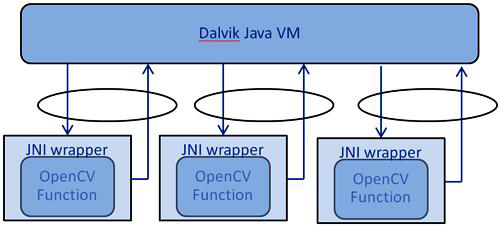
\includegraphics[width=0.85\linewidth]{img/lane12.png}
\caption{When using the Java API}
\label{fig:lane12}
\end{subfigure}
\begin{subfigure}[b]{0.5\textwidth}
\centering
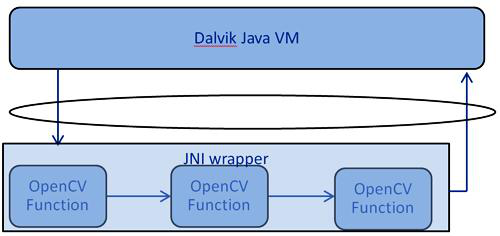
\includegraphics[width=0.85\linewidth]{img/lane13.png}
\caption{Using native C++ to write functions}
\label{fig:lane13}
\end{subfigure}
\end{figure}

\subsection{Class Structure}

Class diagrams represent the structure of classes used in the source code. LineFinder class represent the class which implements the major lane detection and over-laying functions. LaneCalculation class represent functions which are used to calculate lateral position and SDLP values.

\begin{figure}
\begin{center}
    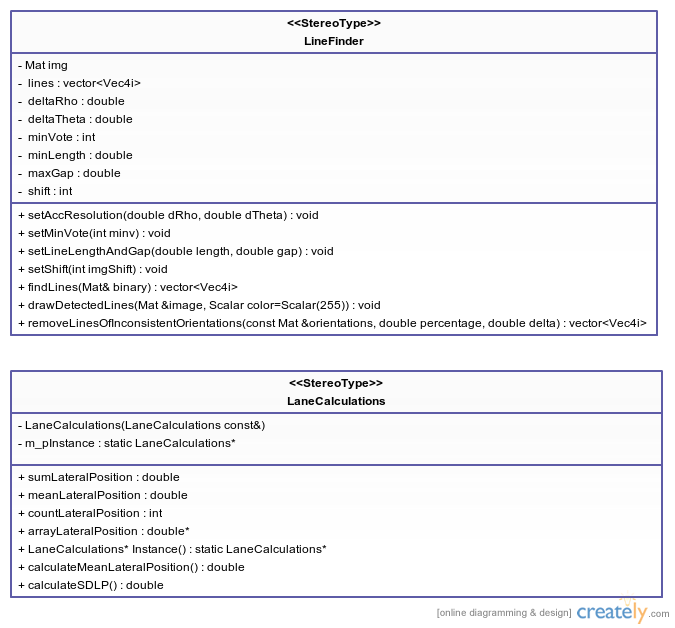
\includegraphics[scale=0.6]{img/lane14.png}
\end{center}
\caption{Class diagrams of main classes}
\end{figure}

\subsection{Optimization and Contributions}

My contribution to the original open source code and optimization techniques which were applied includes :

\begin{itemize}
        \item Creating an Android app, porting the desktop code and customizing it to run on Android NDK
        \item Getting camera input from Android phone in an efficient way using CameraBridgeViewBase class [ref]
        \item Downsampling the input frame by 1/4 before applying computations and then upsampling again before passing it back to JNI wrapper
        \item Using Region of Interest (ROI) by applying a mask and fetching only required area of input and not the whole frame
        \item Adding additional flags in Android.mk and Application.mk files which are used to specify information to Android NDK application
\end{itemize}

I have tested the app on Samsung S5 which is a high-end android phone with quad-core processor. The test case used is the youtube video [6] which is also mentioned previously in the document. Values of Hough Vote were changed using the slider and then once run, frame per second (fps) value is displayed on top left corner of screen. I have used only landscape mode because portrait mode limits the view and we need a good horizontal view of the road. The bar chart shown below shows that fps readings improved significantly after optimization although they are still not very good. The Hough Transform algorithms are very resource intensive. 

\begin{figure}
\begin{center}
    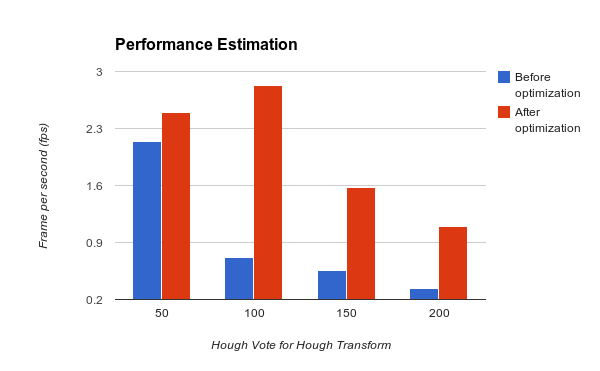
\includegraphics[scale=0.6]{img/lane15.png}
\end{center}
\caption{Class diagrams of main classes}
\end{figure}

\subsection{Issues and Improvements}

This project was a basic prototype or proof of concept developed with many assumptions and certain compromises were made. This is definitely not state-of-the-art solution but can be further used and improved to achieve better results. 

\begin{itemize}
        \item More advanced and better techniques can be incorporated for rapid automated detection of lane boundaries and more accurate overlaying
        \item A technique which can also detect curvatures on lane accurately
        \item A better visualization of lane boundaries and the region in focus to help driver in better understanding of his lane
        \item Improve performance of the app and achieve higher frame per second (fps) rate
\end{itemize}

\subsection{Licenses}

This program is free software; permission is hereby granted to use, copy, modify, and distribute this source code, or portions thereof, for any purpose, without fee, subject to the restriction that the copyright notice may not be removed or altered from any source or altered source distribution. The software is released on an as-is basis and without any warranties of any kind.    In particular, the software is not guaranteed to be fault-tolerant or free from failure. The author disclaims all warranties with regard to this software, any use, and any consequent failure, is purely the responsibility of the user.
